\documentclass[a4paper,12pt]{report}

% Pakete einbinden
\usepackage[utf8]{inputenc}
\usepackage[T1]{fontenc}
\usepackage{lipsum} % für Lorem Ipsum Beispieltext
\usepackage{graphicx} % für Bilder
\usepackage[backend=biber]{biblatex} % für Zitate und Literaturverzeichnis
\addbibresource{bibliography.bib}

\usepackage{minted}
\usepackage[minted]{tcolorbox}


% Custom JavaScript code box with black border
\newtcblisting{code}{
	listing engine=minted,
	listing only,
	minted language=javascript,
	minted style=colorful,
	minted options={
		linenos,
		fontsize=\small,
		breaklines,
		tabsize=2,
		bgcolor=lightgray!25,
	},
	boxrule=0pt,
	top=0pt, bottom=0pt, left=2pt, right=2pt,
	colback=lightgray!25,
}

% Dokumentenbeginn
\begin{document}

% Titelblatt
\title{Titel der Diplomarbeit}
\author{Dein Name}
\date{\today}
\maketitle

% Abstract
\chapter*{Abstract}
\addcontentsline{toc}{chapter}{Abstract}
\lipsum[1]
\newpage

% Abstract
\chapter*{Kurzfassung}
\addcontentsline{toc}{chapter}{Kurzfassung}
\lipsum[1]
\newpage

% Inhaltsverzeichnis
\tableofcontents
\newpage

% Einleitung
\chapter{Introduction}
Link Gliederung: https://www.diplomarbeiten-bbs.at/durchfuehrung/gliederung-der-diplomarbeit-und-formale-vorgaben
\section{Short description}

The topic of this diploma thesis is creating a platform which supports different voting options like single, multiple or weighted choice. Additionally there should be a Login system with different roles to administer and create or delete polls and one where the user can simply vote for the polls he's included in. Furthermore there an option to disclose the results and who voted for which answers. The database should run on a remote server and be accessed by an API. \\
The reason we chose this topic is because our supervisor is part of the LMP party and they couldn't find an appropriate platform to vote on party intern problems and topics. Hence he approached us and suggested we write our diploma thesis on a voting platform.

\section{Description of performed work}
Our aim is to provide a website where different organizations can create and publish polls for their members. Since our finished work will be open source, everyone who wants to create polls will benefit from our work. \\
We chose to accept the LMP as our partner, because they brought up that there isn't a platform that supports all the features they need. Moreover can they give us feedback of the real life application so we can adjust the features to a user organization. During the development of our work we had monthly meetings with the LMP to discuss the progress. Because we decided to develop our software in an agile way the discussions we had with them also helped so we could focus on the more important features first and implement elements of lesser importance later.  

\section{Methodology of the thesis}
At first we had to decide on a tech stack. After careful consideration we decided upon a PostgreSQL database, a backend of node.js, sequelize to perform database operations and express to write APIs so we can connect with our frontend. Our frontend is based on React and we also included a PWA. After this decision we began with a simple input and output from front- to backend so ensure we all understood how each part is connected to each other. The next step was implementing the first features. We split the elements in different components so we could work separately and efficiently, e.g the single choice is split in create the poll, display the poll, vote, and show the results. Reasons we chose this tech stack and a thorough description of each function our work has will be in the main part.  
% Beispielbild einfügen
\begin{figure}[h!]
    \centering
    
\includegraphics[width=0.5\textwidth]{pics/beispiel.jpg}
    \caption{Hier ist ein Bier}
    \label{fig:beispielbild}
\end{figure}

% Hauptteil
\chapter{Tech Stack}
\section{PostgreSQL}
\section{node.js}
\section{Sequelize}
\section{express}
\section{React}
\section{PWA}
\chapter{Features}
\begin{figure}[h!]
\begin{code}
useEffect(() => {
	const linkParam = window.location.search.substring(1);
	if (linkParam) {
		const unhashed = atob(decodeURIComponent(linkParam));
		const params = new URLSearchParams(unhashed);
		const token = params.get('token');
		if (token) {
			setNewUserRegistration(1);
			setNewUserToken(token);
		} else {
			const publicValue = params.get('public');
			if (publicValue === "true") {
				setIsPublic(1);
			} else {
				setIsPublic(0);
			}
		}
	}
}, []);
\end{code}
	\caption{Hier ist ein Beispielcode}
	\label{fig:beispielcode}
\end{figure}
\begin{figure}[h!]
	\begin{code}
		useEffect(() => {
			const linkParam = window.location.search.substring(1);
			if (linkParam) {
				const unhashed = atob(decodeURIComponent(linkParam));
				const params = new URLSearchParams(unhashed);
				const token = params.get('token');
				if (token) {
					setNewUserRegistration(1);
					setNewUserToken(token);
				} else {
					const publicValue = params.get('public');
					if (publicValue === "true") {
						setIsPublic(1);
					} else {
						setIsPublic(0);
					}
				}
			}
		}, []);
	\end{code}
	\caption{Hier ist ein Beispielcode}
	\label{fig:beispielcode2}
\end{figure}

\section{Login}
\section{Registration}
\subsection{Roles}
Implementing a role-based system with three distinct roles - "Admin," "Poweruser," and "Normal" - is crucial for te functionality and security of the application. By assigning permissions flexibly, a clear hierarchy is established, enhancing both user experience and data integrity. Admins are grated full control over the application, while Poweruser enjoy extended privileges for managing polls. Normal users can seamlessly participate in polls and view results without jeopardizing sensitive functionalities. This structure facilitates efficient task delegation an scalability, allowing the application to be easily expanded with additional roles  in the future. The role system thus significantly contributes to the security, organization, and user-friendliness of the polling application.
\section{Group System}
\section{Create Polls}
\subsection{Start-/ Endtime}
\subsection{Questions}
\subsubsection{Single Choice}
\subsubsection{Multiple Choice}
\subsubsection{Weighted Choice}
\subsection{Demographic Questions}
\paragraph{}
To gather the data of our public voters, the implementation of demographic questions was crucial. This feature is only available for public polls since the created user would be part of the organization using our project and therefore have the data already. If the users is not part of the organization there is still the option to contact them via the e-mail used for the registration. Since most of these questions are similar for every poll, a modular system where questions can be created, added, removed and changed is the best solution. Figure \ref{fig:create_dem_que} shows the demographic question in create polls. The options and functionality of these questions are the like ones described in the previous sections. 
\begin{figure}[h!]
	\centering
	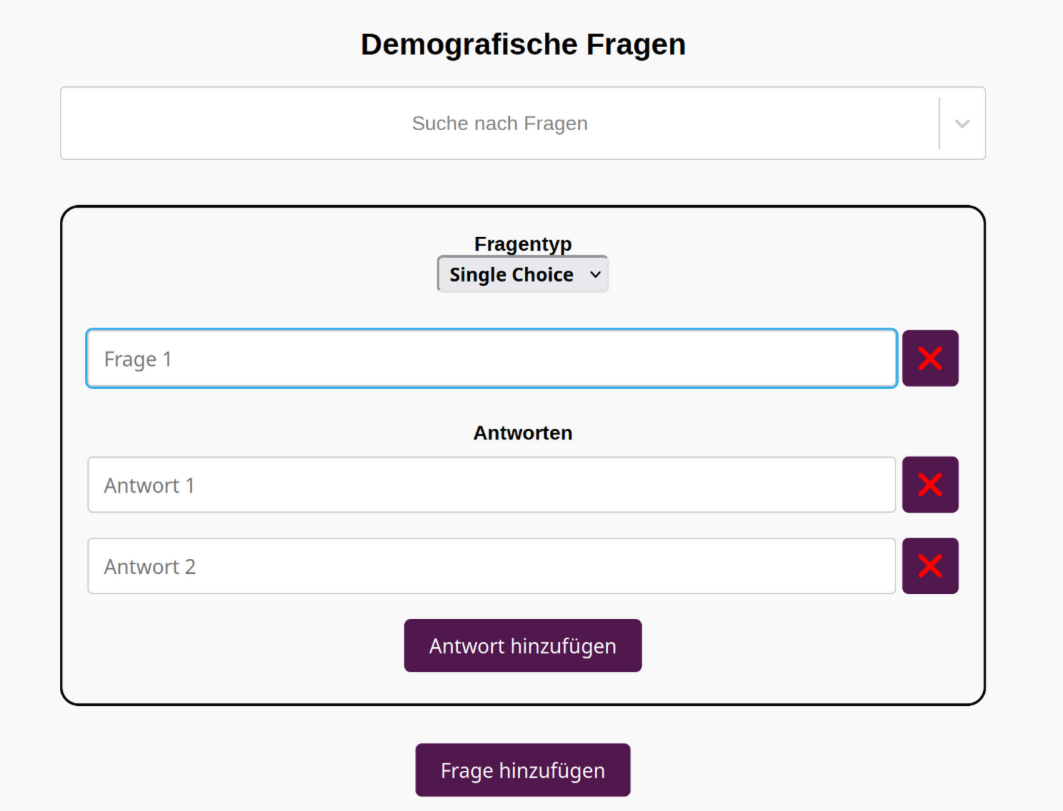
\includegraphics[width=0.6\textwidth]{pics/demographic_question_create.jpg}
	\caption{Create Demographic Question}
	\label{fig:create_dem_que}
\end{figure}
\paragraph{}
The new part for this feature is the search bar. For this the "Select" component of "react-select" is used. The components' controllable state props and modular architecture allows  "isMulti" to select multiple options or "isSearchable" to search. These features, allow easy implementation and an already styled search bar in the project. \parencite{reactselect}
\paragraph{}
The database structure for the demographic questions is similar to the standard ones. The table "PublicQuestions" is used to store the question specific data like name and type. To enable the reuse of questions on different polls "PublicQuestions" is in an many-to-many relationship with "Polls" through "PublicPollQuestions". Answers are stored within the table "PublicAnswers", which is connected to "PublicQuestions" via "PublicQuestionAnswers. This relation is also many-to-many since the options yes or no for example would be used in multiple questions. 
\paragraph{}
For the select every existing question with its answers is fetched from the database and stored within an array. The options are then mapped with the value being id and the label as name of each element. To display the selected options they are mapped through and use the same functions as the standard ones used for the poll. When saving these questions a problem arises, as the selected ones are already stored in the database and possibly changed. To handle this an findOrCreate \ref{fig:publicQuestions} is used to get the existing questions and answers or create new ones. This function also returns each instance found or the created one. With this the question and answer ids can be used for the many-to-many relationship. \parencite{sequelizedoku} 
\begin{figure}[h!]
\begin{code}
let [createdQuestion, created] = await PublicQuestions.findOrCreate({
	where: {
		name: question.name,
		typeId: questionType.id,
	}
});
\end{code}
	\caption{findOrCreate PublicQuestions}
	\label{fig:publicQuestions}
\end{figure}

\section{Edit Polls}
\section{Voting}
\subsection{Disclosed Voting}
\subsection{Anonymous Voting}
\subsection{Public Voting}
The public voting allows users without an account to vote. With this feature a wide range of people can be questioned via street surveys or through a shared link. This poll type has two section, the normal and demographic questions. The order of these play a major role. \textcite{demographicdata} mentions trust, benefits of the demographic data and the ability to abstain. All of these factors have to be taken into ones account when creating these questions. The article also mentions, that at the beginning of a survey the motivation is high and the demographic data are answered, but the trust in full anonymity is decreased. Therefore the author states it is best to put these questions at the end. 
\subsubsection{Vote integrity}
A major problem when having anonymity and no accounts is the data integrity. Without the ability to store information about a voter in the database to check for multiple votes, it is important to prevent them from voting multiple times.  

what to write about:
how to prevent multiple votes: 
- 	captcha against bots 
-	cookies to prevent non techie users 
-	users with knowledge almost impossible to prevent without storing ip or device fingerprints, 
problem with ip and device fp is probably legal reasons

-	userData: which information is important for polls (gender, age, job, )

\section{Results}
\subsection{CSV-Export}
\section{MyPolls}
\subsection{Polllink}
\subsection{Delete Polls}
\section{Accessibility}
\subsection{Tooltips}
\subsection{Screenreader}
\section{Styling}
\chapter{Summary}
\lipsum[1]

% Literaturverweis-Beispiel
Hier ein Zitat aus einer Quelle \cite{author2023example}.

% Zusammenfassung


% Literaturverzeichnis
\printbibliography

% Abbildungsverzeichnis
\listoffigures
\newpage

\end{document}
